\section{Comparison of Solver Concepts}
  
\subsection{Convergence Behaviour on Locally Refined Block Structured Grids with Different Degrees of Coupling}

Show how the implicit treatment of block boundaries maintains (high) convergence rates. Plot Residual over number of iterations. Plot Wall time for a single block using SIP, KSP, COUPLED for different grid resolutions.

\subsection{Parallel Performance}

In many cases, scientific code is used to solve complex problems regarding memory requirements to make calculation results available within short time. In both scenarios, code that is able to run in parallel can alleviate the mentioned challenges. Code that runs in parallel can allocate more memory resources which makes the calculation of complex problems feasible. If the code is scalable the program execution can be shortened by using more processors to solve a problem of constant size.

The solver framework that has been developed in the course of the present thesis, has been parallelized using the PETSc library. After introducing the used hardware and software, the central measures of parallel performance are presented. Then preliminary test results using low-level benchmarks are performed, which establish upper performance bounds on the parallel efficiency and the scalability of the developed solver framework. The results of the efficiency evaluation of the solver framework is presented in the last subsections.
\subsubsection{Employed Hardware and Software -- The Lichtenberg-High Performance Computer }

All performance analyses that are presented in this thesis were conducted on the Lichtenberg-High Performance Computer, also known as \emph{HHLR} (\emph{Hessischer Hochleistungsrechner}) \cite{hhlr}. The cluster consist of different sections according to the used hardware. Throughout the thesis, tests were performed using the first and the second MPI section of the cluster. The first section consists of 705 nodes of which each runs two Intel\textregistered Xeon\textregistered E5-2670 processors and offers 32GB of memory. The second section consists of 356 nodes of which each runs two Intel Xeon E5-2680 v3 processors and offers 64GB of memory. As interconnect for both sections FDR-14 InfiniBand is used.

All tests programs were compiled using the Intel compiler suite version 15.0.0 and the compiler options
\lstset{language=bash,
  commentstyle={\rmfamily\catcode`\$=11},
  columns=flexible,
  texcl,
  keepspaces,
  ,showspaces=false
  ,showstringspaces=false,
  }
\begin{lstlisting}
-O3 -xHost
\end{lstlisting}
As MPI implementation Open MPI version 1.8.2 was chosen. Furthermore the PETSc version 3.5.3 was configured using the options
\begin{lstlisting}
--with-blas-lapack-dir=/shared/apps/intel/2015/composer_xe_2015/mkl/lib/intel64/ \
--with-mpi-dir=/shared/apps/openmpi/1.8.2_intel \
COPTFLAGS="-O3 -xHost" \
FOPTFLAGS="-O3 -xHost" \
CXXOPTFLAGS="-O3 -xHost" \
--with-debugging=0 \
--download-hypre \
--download-ml
\end{lstlisting}
It should be noted that as the configurations options show, to maximize the efficiency of PETSc, a math kernel library should be used that has been optimized for the underlying hardware architecture as is in the case of the present thesis the Intel \emph{MKL} (\emph{Math Kernel Library}). It should be noted that also the Open MPI library has been compiled using the Intel compiler suite.

\subsubsection{Measures of Performance}

This section establishes the needed set of measures to evaluate the performance of a solver program, which will be used in the following sections. The first measure is the plain measure of runtime \(T_P\) taken by a computer to solve a given problem, where \(P \in \mathbb{N}\) denotes the number of involved processes. This so called \emph{wall-clock} time can be measured directly by calling subroutines of the underlying operating system and corresponds to the human perception of the time, that has passed. It must be noted, that this time does not correspond to the often mentioned \emph{CPU} time. In fact, CPU time is only one contributor to wall-clock time. Wall-clock time further contains the time needed for communication and I/O and hence considers idle states of the processor. On the other side CPU time only considers the time in which the processor is actively working. This makes wall-clock time not only a more complete but also more accurate time measure when dealing with parallel processors, since processor idle times due to communication are actively considered while neglected in CPU time.

While wall-clock time is an absolute measure that can be used to compare different solver programs, further relative measures are needed to evaluate the efficiency of one program regarding the parallelisation implementation. The main purpose of these measures is to attribute the different causes of degrading efficiency due to heavy parallelisation to the different contributing factors. A simple model \cite{ferziger02,schaefer99} considers three contributions, that form the total efficiency
\begin{displaymath}
  E^{tot}_P = E^{num}_P \cdot E^{par}_P \cdot E^{load}_P.
\end{displaymath}
\begin{itemize}
  \item[] The \emph{numerical efficiency}
  \begin{displaymath} E^{num}_P := \frac{\operatorname{FLOPS}(1)}{P \cdot \operatorname{FLOPS}(P)}\end{displaymath} 
    considers the degradation of the efficiency of the underlying algorithm due to the parallelisation. Many efficient algorithms owe their efficiency to recursions inside the algorithm. In the process of decomposing this recursions, the efficiency of the algorithm degrades. It follows that this efficiency is completely independent of the underlying hardware.
  \item[] The \emph{parallel efficiency}
    \begin{displaymath} E^{par}_P :=\frac{\operatorname{TIME}(\text{parallel Algorithm on one processor})}{P \cdot \operatorname{TIME}(\text{parallel Algorithm on \(P\) processors})} \end{displaymath} 
      describes the impact of the need for inter process communication, if more than one processor is involved in the solution process. It should be noted, that this form of efficiency does explicitly exclude any algorithm related degrading, since the time measured corresponds to the exact same algorithms. It follows that the parallel efficiency only depends on the implementation of the communication and the hardware related latencies.
  \item[] The \emph{load balancing efficiency} 
    \begin{displaymath} E^{load}_P :=\frac{\operatorname{TIME}(\text{calculation on complete domain})}{P \cdot \operatorname{TIME}(\text{calculation on biggest subdomain})} \end{displaymath}
       is formed by the quotient of the wall times needed for the complete problem domain and partial solves on subdomains. This measure does neither depend on hardware nor on the used implementation. Instead it directly relates to the size and partition of the grid. 
\end{itemize}

It is not possible to calculate all three efficiencies at the same time using only plain wall clock time measurements of a given application.  Different solver configurations have to be used to calculate them separately. Since the focus of investigation of the present thesis does not lie on load balancing, for the remainder of the thesis \(E^{load}_P = 100\%  \) is assumed. This does not present a considerable drawback, since an ideal load balancing is easily obtainable nowadays by the use of sophisticated grid partitioning algorithms \cite{loadbalancing} REFERENCES. Using identical algorithms for different numbers of involved processes implicitly achieves \(E^{num}_P = 100 \%\). In this case the parallel efficiency of an application can be measured through the quotient of the needed wall clock time. To measure the numerical efficiency of an algorithm the respective hardware counters have to be evaluated. This can be done using the built in log file functionality of PETSc as presented in section REFERENCE. Hence the determination of numerical efficiency does not rely on wall clock time.

Another common performance measure is the \emph{Speed-Up}
\begin{displaymath}
  S_P = \frac{T_1}{T_P} = P \cdot E^{tot}_P.
\end{displaymath}
Speedup and parallel efficiency characterize the parallel scalability of an application and determine the regimes of efficient use of hardware resources.

\subsubsection{Preliminary Upper Bounds on Performance -- The STREAM Benchmark}

Scientific applications that solve partial differential equations rely on sparse matrix computations, which usually exhibit the sustainable memory bandwidth as bottleneck with respect to the runtime performance of the program \cite{hager11}. The purpose of this section is to establish a frame in terms of an upper bound on performance in which the efficiency of the developed solver framework can be evaluated critically. As common measure for the maximum sustainable bandwidth, low-level benchmarks can be used, which focus on evaluating specific properties of the deployed hardware architecture. In this case the STREAM benchmark suite \cite{mccalpin07,mccalpin95} provides apt tests, which are designed to work with data sets that exceed the cache size of the involved processor architecture. This forces the processors to stream the needed data directly from the memory instead of reusing the data residing in their caches. These types of tests can be used to calculate an upper bound on the memory bandwidth for the CAFFA framework.

In terms of parallel scalability, the STREAM benchmark can also be used as an upper performance bound. According to \cite{petsc-web-page} the parallel performance of memory bandwidth limited codes correlates with the parallel performance of the STREAM benchmark, i.e. a scalable increase in memory bandwidth is necessary for scalable application performance. The intermediate results of the benchmark can then be used to test different configurations that bind hardware resources to the involved processes. Before presenting results the different binding configurations will be explained.

The first configuration sequentially binds the processes to the cores beginning on the first socket. When every core has a bound process the binding algorithm binds the following processes to cores of the second socket. The second configuration binds the processes in a round robin manner regarding the sockets. This configuration in difference to the second configuration binds one process to three cores. Figures \ref{fig:binding1},\ref{fig:binding2} and \ref{fig:binding3} demonstrate the different binding options for two sockets and processors with twelve cores each, when eight processes are to be bound to the resources.

\begin{figure}[h]
  \centering
  \label{fig:binding1}
    \input{./img/map2.tikz.tex}
    \centering{}
  \caption{Default binding using Open MPI on a node with two sockets and processors with each twelve cores}
\end{figure}

\begin{figure}[h]
  \centering
  \label{fig:binding2}
    \newcommand*{\xMin}{0}%
\newcommand*{\xMax}{12}%
\newcommand*{\yMin}{0}%
\newcommand*{\yMax}{1}%
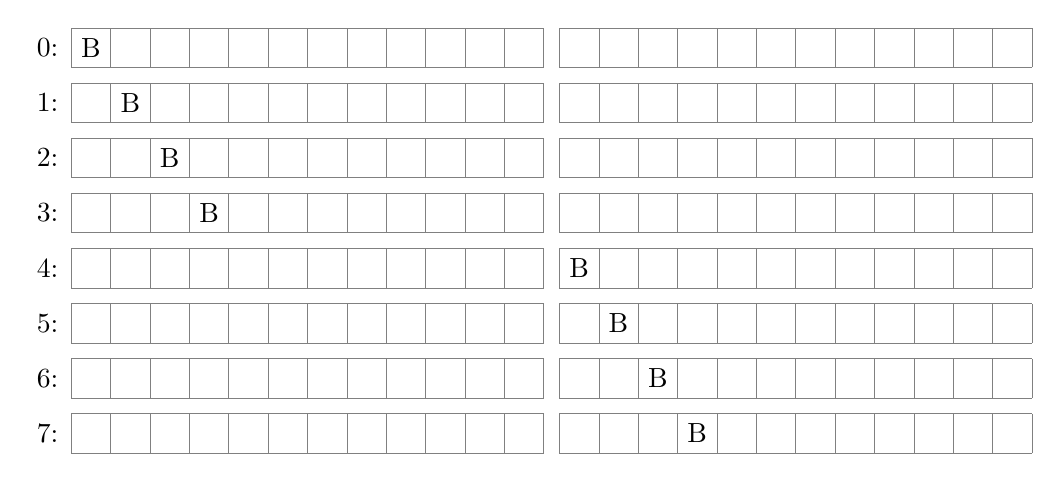
\begin{tikzpicture}
%   \foreach \i in {\xMin,...,\xMax} {
%       \draw [very thin,gray] (\i,\yMin) -- (\i,\yMax)  ;
%   }
%   \foreach \i in {\yMin,...,\yMax} {
%       \draw [very thin,gray] (\xMin,\i) -- (\xMax,\i) ;
%   }
    \foreach \j in {0,0.7,1.4,2.1,2.8,3.5,4.2,4.9} {
    \foreach \i in {0,0.5,1.0,1.5,2.0,2.5,3.0,3.5,4.0,4.5,5.0,5.5,6.0} {
        \draw [very thin,gray] (\i,\j) -- (\i,\j+0.5)  ;
        }

    \foreach \i in {\j,\j+0.5} {
        \draw [very thin,gray] (0,\i) -- (6.0,\i)  ;
        }


    \foreach \i in {0,0.5,1.0,1.5,2.0,2.5,3.0,3.5,4.0,4.5,5.0,5.5,6.0} {
        \draw [very thin,gray] (\i+6.2,\j) -- (\i+6.2,\j+0.5)  ;
        }

    \foreach \i in {\j,\j+0.5} {
        \draw [very thin,gray] (6.2,\i) -- (12.2,\i)  ;
        }
    }

    \node at (-0.3,0.25) {7: };
    \node at (-0.3,0.95) {6: };
    \node at (-0.3,1.65) {5: };
    \node at (-0.3,2.35) {4: };
    \node at (-0.3,3.05) {3: };
    \node at (-0.3,3.75) {2: };
    \node at (-0.3,4.45) {1: };
    \node at (-0.3,5.15) {0: };
    \node at (0.25,5.15) {B};
    \node at (0.75,4.45) {B};
    \node at (1.25,3.75) {B};
    \node at (1.75,3.05) {B};
    \node at (0.25+6.2,2.35) {B};
    \node at (0.75+6.2,1.65) {B};
    \node at (1.25+6.2,0.95) {B};
    \node at (1.75+6.2,0.25) {B};

  

\end{tikzpicture}

    \centering{}
  \caption{Process binding using Open MPI and map-by ppr:8:node map-by ppr:4:socket on a node with two sockets and processors with each twelve cores}
\end{figure}


\begin{figure}[h]
  \centering
  \label{fig:binding3}
    \input{./img/map3.tikz.tex}
    \centering{}
  \caption{Process binding using Open MPI and map-by ppr:8:node map-by ppr:4:socket:PE=3 on a node with two sockets and processors with each twelve cores}
\end{figure}

\begin{figure} \centering
  \pgfplotsset{every axis/.append style={
      font=\large,
      line width=1pt,
  tick style={line width=0.8pt}}}
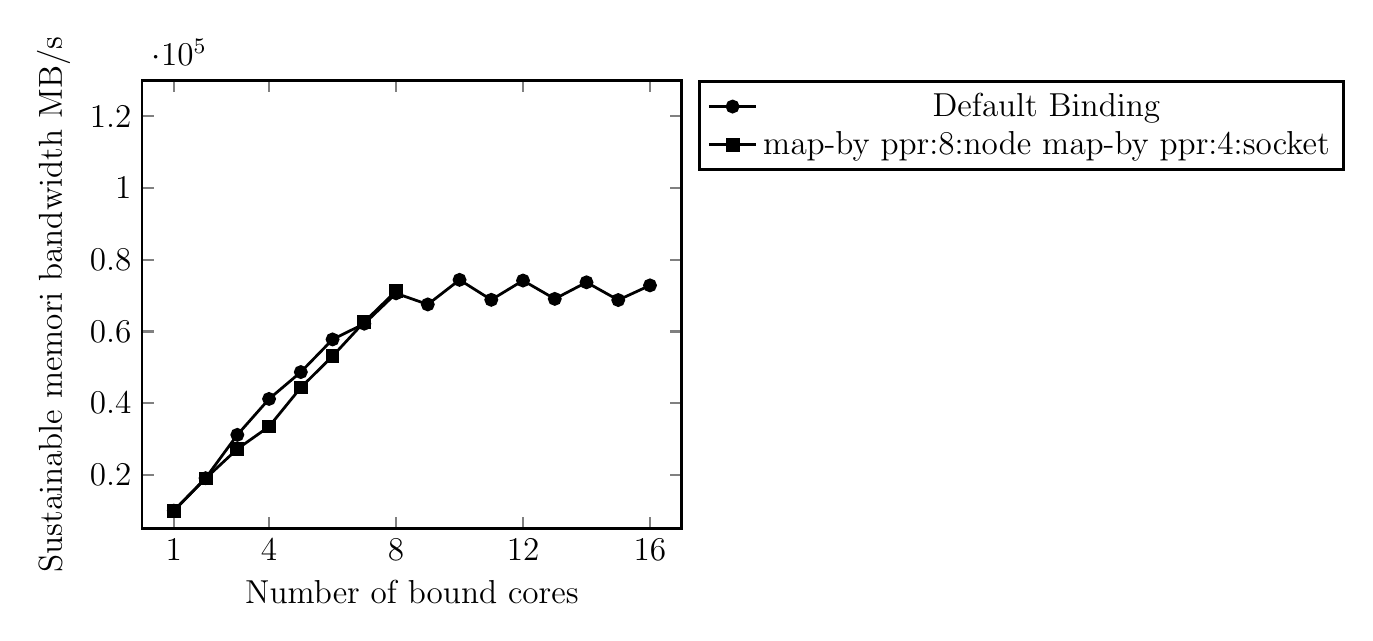
\begin{tikzpicture}
\begin{axis}[
    ylabel={Sustainable memori bandwidth MB/s},
    xlabel={Number of bound cores},
    xtick={1,4,8,12,16},
    %ytick={1.7e-003,1.75e-3,1.8e-003,1.85e-3},
    %yticklabels={1.7E-3,1.75E-3,1.8E-3,1.85E-3},
    %ymin=1.65e-003,ymax=1.9e-003,
    xmin=0,xmax=17,
    ymin=0.5e4,ymax=1.3e5,
    legend pos=outer north east,
    %height=20cm,width=10cm
    ]
    \addplot[color=black,mark=*] coordinates {
        (1,10056.2733)
        (2,19114.3429)
        (3,31197.8399)
        (4,41210.0612)
        (5,48699.7232)
        (6,57803.5686)
        (7,62187.9785)
        (8,70658.3730)
        (9,67558.4259)
        (10,74413.8457)
        (11,68849.0631)
        (12,74223.3175)
        (13,69109.0762)
        (14,73729.0608)
        (15,68784.2613)
        (16,72872.4480) };
        \addlegendentry{Default Binding};
    \addplot[color=black,mark=square*] coordinates {
        (1 ,10044.2323)
        (2 ,19036.1755)
        (3 ,27258.6888)
        (4 ,33509.0570)
        (5 ,44386.9342)
        (6 ,53130.5978)
        (7 ,62695.4511)
        (8 ,71295.7113) };
        \addlegendentry{map-by ppr:8:node map-by ppr:4:socket}
\end{axis}
\end{tikzpicture}
\caption{Sustainable memory bandwidth as determined by the STREAM benchmark (Triad) for different process binding options on one node of the MPI1 section}
\end{figure}

\begin{figure} \centering
  \pgfplotsset{every axis/.append style={
      font=\large,
      line width=1pt,
  tick style={line width=0.8pt}}}
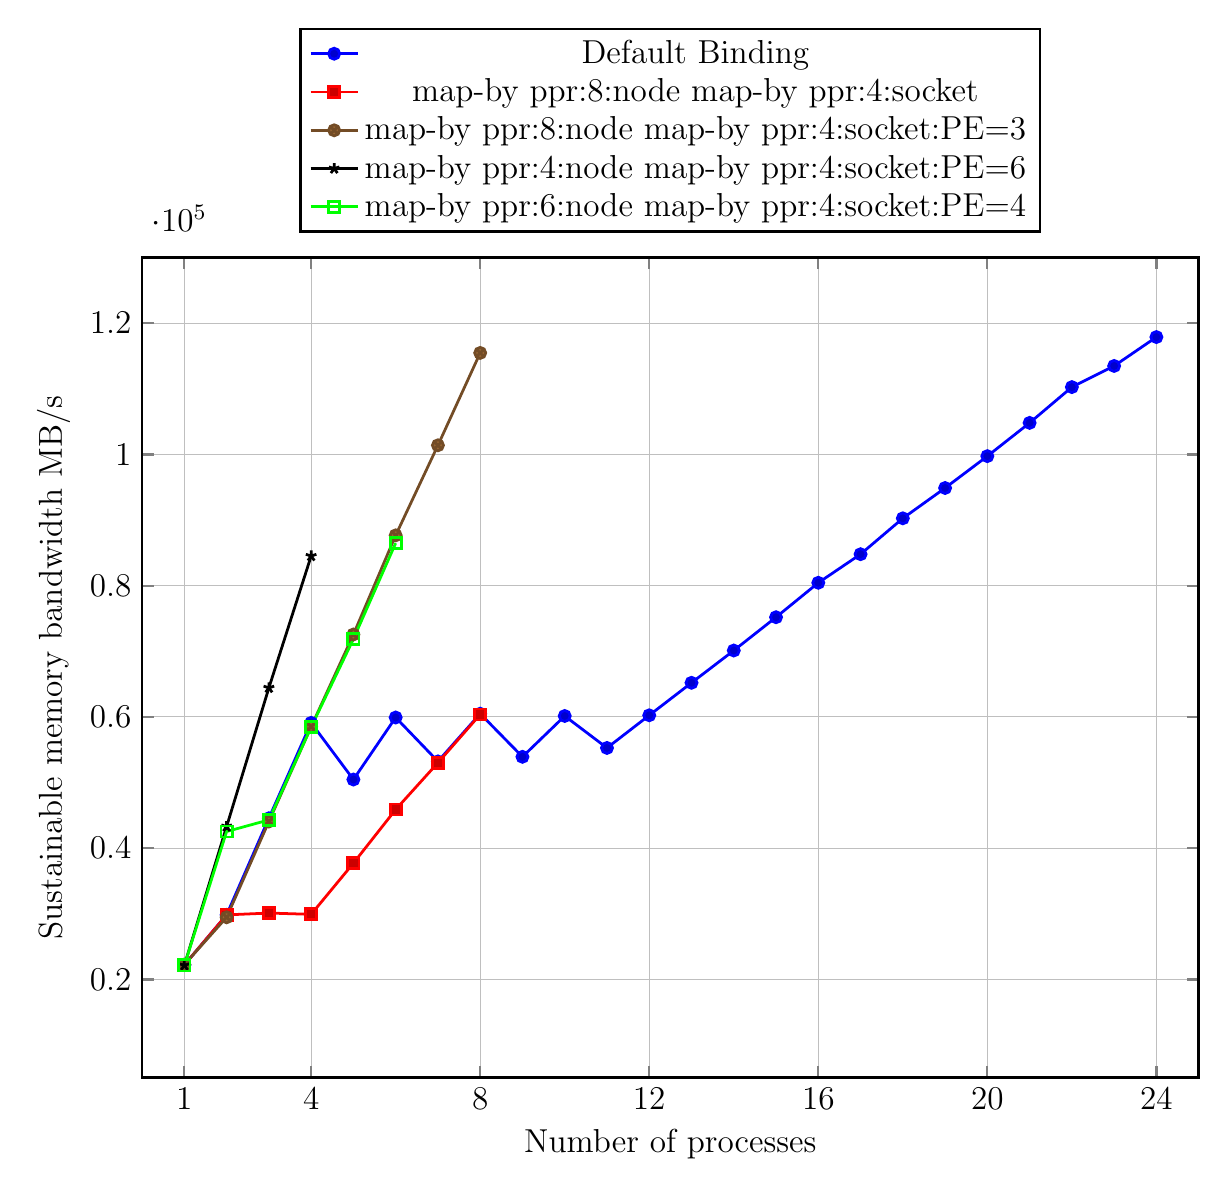
\begin{tikzpicture}
  \pgfplotsset{every axis legend/.append style={
      at={(0.5,1.03)},
  anchor=south}}
\begin{axis}[
    ylabel={Sustainable memory bandwidth MB/s},
    xlabel={Number of processes},
    xtick={1,4,8,12,16,20,24},
    %ytick={1.7e-003,1.75e-3,1.8e-003,1.85e-3},
    %yticklabels={1.7E-3,1.75E-3,1.8E-3,1.85E-3},
    %ymin=1.65e-003,ymax=1.9e-003,
    xmin=0,xmax=25,
    ymin=0.5e4,ymax=1.3e5,
    height=12cm,width=15cm,
    grid=major,
    ]
    \addplot coordinates {
           
      (1, 22201.8738 )
      (2,    29846.0651 )
      (3,    44558.8130 )
      (4,    59096.4718 )
      (5,    50460.8297 )
      (6,    59912.1938 )
      (7,    53222.7910 )
      (8,    60491.6764 )
      (9,    53922.4875 )
      (10,    60144.1732 )
      (11,    55273.7403 )
      (12,    60248.1185 )
      (13,    65200.5600 )
      (14,    70118.7250 )
      (15,    75192.3175 )
      (16,    80439.8917 )
      (17,    84793.6761 )
      (18,    90263.9931 )
      (19,    94881.4421 )
      (20,    99735.0136 )
      (21,   104804.3772 )
      (22,   110256.7754 )
      (23,   113478.3185 )
      (24,   117880.3816 ) };
     \addlegendentry{Default Binding};
     \addplot coordinates{
       (1, 22211.6717)
       (2, 29836.1141)
       (3, 30113.6704)
       (4, 29919.5219)
       (5, 37713.7578)
       (6, 45888.1496)
       (7, 53019.1276)
     (8, 60375.4338) };
     \addlegendentry{map-by ppr:8:node map-by ppr:4:socket};
     \addplot coordinates{
       (1, 22265.7147)
       (2, 29467.1111)
       (3, 44064.6918)
       (4, 58503.9143)
       (5, 72560.6185)
       (6, 87667.8368)
       (7,101388.5503)
     (8,115464.4300) };
     \addlegendentry{map-by ppr:8:node map-by ppr:4:socket:PE=3};
     \addplot coordinates{
       (1, 22140.8327)
       (2, 43291.3883)
       (3, 64431.3899)
      (4, 84515.5468) };
      \addlegendentry{map-by ppr:4:node map-by ppr:4:socket:PE=6};
      \addplot[color=green,mark=square] coordinates{
        (1,22140.8327)
        (2,42536.7826)
        (3,44307.1664)
        (4,58452.9712)
        (5,71870.5626)
        (6,86478.5257)
      };
      \addlegendentry{map-by ppr:6:node map-by ppr:4:socket:PE=4};
\end{axis}
\end{tikzpicture}
\caption{Sustainable memory bandwidth as determined by the STREAM benchmark (Triad) for different process binding options on one node of the MPI2 section}
\end{figure}

\subsubsection{Optimization of Sequential Solver Configuration}

Compare runtime for different solver configurations BiCGStab+ICC, different multigrid algorithms

\subsubsection{Evaluation of Numerical Efficiency of the Solver Algorithm}
\subsubsection{Discussion of Results for Parallel Efficiency}

\subsubsection{Speedup Measurement for Analytic Test Cases}

\subsection{Test Cases with Varying Degree of Non-Linearity}
      
As Peric says I want to prove that the higher the non-linearity of NS, the better relative convergence rates can be achieved with a coupled solver. Fi

\subsubsection{Transport of a Passive Scalar -- Forced Convection}
\subsubsection{Buoyancy Driven Flow -- Natural Convection}
\subsubsection{Flow with Temperature Dependent Density -- A Highly Non-Linear Test Case}
Maybe I could consider two test cases, one with oscillating density and one with a quadratic polynomial. Interesting would be also to consider the dependence of convergence on another scalar transport equation

\subsection{Realistic Testing Scenarios -- Benchmarking}
Also consider simple load balancing by distributing matrix rows equally

\subsubsection{Flow Around a Cylinder 3D -- Stationary}
Describe Testing Setup (Boundary conditions and grid). Present results and compare them with literature.
\subsubsection{Flow Around a Cylinder 3D -- Instationary}
\begin{itemize}
\item\url{http://www.featflow.de/en/benchmarks/cfdbenchmarking/flow/dfg_flow3d/dfg_flow3d_configuration.html}
\end{itemize}
Describe Testing Setup (Boundary conditions and grid). Present results and compare them with literature.
      \subsubsection{Heat-Driven Cavity Flow}
      \begin{itemize}
      \item \url{http://www.featflow.de/en/benchmarks/cfdbenchmarking/mit_benchmark.html}
      \end{itemize}
      Describe Testing Setup (Boundary conditions and grid). Present results and compare them with literature.
\subsection{Realistic Testing Scenario -- Complex Geometry}
